\section{Auswertung}
\label{sec:Auswertung}

Im Folgenden werden die Messungen, dargestellt in \autoref{fig:kurve1} bis \autoref{fig:kurve4}, ausgewertet.
Dafür wird zunächst die mittlere freie Weglänge bestimmt.
Dann wird die Energieverteilung der beschleunigten Elektronen errechnet, indem die Bremsspannung variiert wird.
Schließlich werden die beiden Franck-Hertz-Kurven ausgewertet.


\subsection{Die mittlere freie Weglänge}
Mit \autoref{eq:druck1} und \autoref{eq:u1} wird die mittlere freie Weglänge der beschleunigten Elektronen,
die aus der Heizkathode herausgelöst werden, berechnet.
Ebenfalls wird das Verhältnis $a / \bar{\omega}$ bestimmt.
Die Ergebnisse der Rechnung sind in \autoref{tab:tabelle1} dargestellt.

\begin{table} [H]
  \centering
  \caption{Die mittlere freie Weglänge.}
  \label{tab:tabelle1}
  \begin{tabular}{c c c}
      \toprule
      Temperatur $T \mathbin{/} \unit\kelvin$ & $\bar{\omega} \mathbin{/} \unit\meter$ & $a \mathbin{/} \bar{\omega}$ \\
      \midrule 
      298,35 & 0,538412049 &  0,01857314\\
      433,25 & 0,000411729 & 24,2877893\\
      448,55 & 0,000239611 & 41,7343021\\
      459,05 & 0,000168744 & 59,2613673\\
      \bottomrule
  \end{tabular}
\end{table}

\subsection{Differentielle Energieverteilung}
Nun werden die Messdaten der ersten beiden Messungen ausgewertet.
Dabei handelt es sich um \autoref{fig:kurve1} und \autoref{fig:kurve2}, wobei die Graphen von einem XY-Schreiber erstellt wurden.
Die Beschleunigungsspannung wird zunächst konstant mit $U_\text{B} = \qty{11}{V}$ gewählt.

\subsubsection*{Messung bei 298,35 Grad Kelvin}
Um die Energieverteilung in Abhängigkeit der Spannung zu erhalten, wird das Verhältnis von $\frac{\increment y}{\increment x}$ gebildet.
Dabei kann $y$ in Skalenanteilen angegeben werden.
Als ein Skalenanteil wird ein Kästchen des Millimeter Papiers gewählt.
Die Werte sind in \autoref{tab:tabelle2} angegeben, beziehungsweise in \autoref{fig:plot1} abgebildet.
Es lässt sich erkennen, dass die Steigung den größten Abfall bei $U_\text{B, eff} = \qty{7.75}{V}$ hat.
Damit haben die meisten Elektronen eine Energie in Beschleunigungsrichtung von $E = \qty{7.75}{eV}$.
Schließlich lässt sich noch das Kontaktpotential mit \autoref{eq:Kontaktpotential} zu
\begin{equation}
  K = \frac{\left( \Phi_\text{B} - \Phi_\text{G} \right)}{e_0} = U_\text{B} - U_\text{B, eff} = (11 - 7,75) \, \unit\V = \qty{3.25}{V}
\end{equation}
angeben.
% \begin{table} [H]
%   \centering
%   \caption{Die mittlere freie Weglänge.}
%   \label{tab:tabelle2}
%   \begin{tabular}{c c c}
%       \toprule
%       $U / \unit\V$ & $\frac{y}{\text{Skt}_y}$ & $m  =\frac{y_{i+1} - y_{i}}{U_{i+1} - U_{i}}$ \\
%       \midrule 
%       0   & 15.8  &  -  \\
%       1   & 14.1  & -1.7\\
%       2   & 12.6  & -1.5\\
%       3   & 11.1  & -1.5\\
%       4   & 9.6   & -1.5\\
%       5   & 7.8   & -1.8\\
%       6   & 6     & -1.8\\
%       7   & 4     & -2. \\
%       7,5 & 2.8   & -2.4\\
%       7,75& 1,5   & -5.2\\
%       8   & 0.8   & -2.8\\
%       9   & 0.3   & -0.5\\
%       10  & 0.3   & 0.  \\
%       \bottomrule
%   \end{tabular}
% \end{table}

% \begin{figure}
%   \centering
%   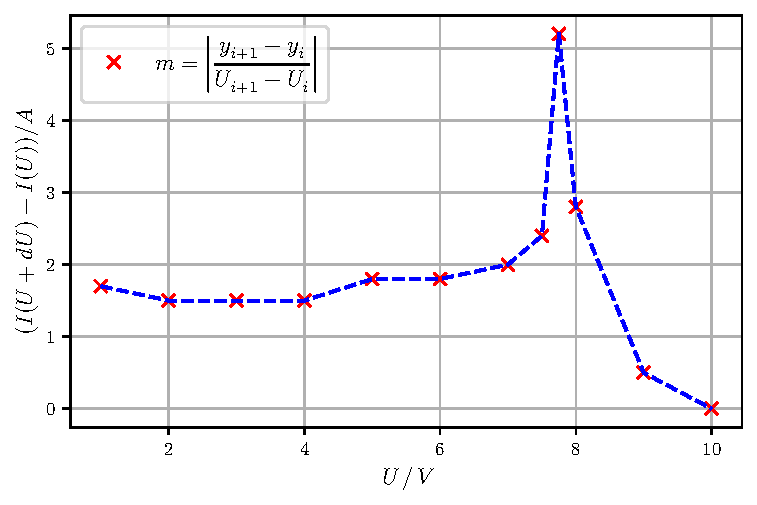
\includegraphics[width=0.5\linewidth]{build/plot1.pdf}
%   \caption{Die Steigung in Abhängigkeit der Spannung.}
% \end{figure}

\begin{table}[H]
  \begin{minipage}[b]{0.4\linewidth}
    \centering
    \begin{tabular}{c c c}
      \toprule
      $U / \unit\V$ & $\frac{y}{\text{Skt}_y}$ & $m  =\frac{y_{i+1} - y_{i}}{U_{i+1} - U_{i}}$ \\
      \midrule 
      0,0 & 15,8  &  -   \\
      1,0 & 14,1  & -1,7 \\
      2,0 & 12,6  & -1,5 \\
      3,0 & 11,1  & -1,5 \\
      4,0 &  9.6  & -1,5 \\
      5,0 &  7.8  & -1,8 \\
      6,0 &  6,0  & -1,8 \\
      7,0 &  4,0  & -2,0 \\
      7,5 &  2,8  & -2,4 \\
      7,75&  1,5  & -5,2 \\
      8,0 &  0,8  & -2,8 \\
      9,0 &  0,3  & -0,5 \\
      10,0&  0,3  &  0,0 \\
      \bottomrule
    \end{tabular}
    \caption{Die gem. Messwerte bei $\qty{298.35}{°K}$.}
    \label{tab:tabelle2}
  \end{minipage}\hfill
  \begin{minipage}[b]{0.45\linewidth}
  \centering
  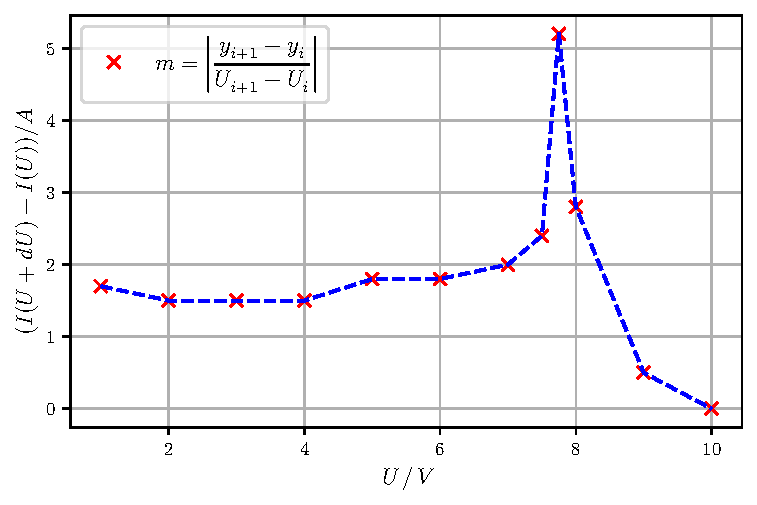
\includegraphics[width=\linewidth]{build/plot1.pdf}
  \captionof{figure}{Die Steigung in Abhängigkeit der Spannung.}
  \label{fig:plot1}
  \end{minipage}
\end{table}

\subsubsection*{Messung bei 433,25 Grad Kelvin}

Bei der Messung mit $\qty{433.25}{°K}$ ergeben sich die Messwerte in \autoref{tab:tabelle3}.
Die Steigung wird dann gegen die Bremsspannung in \autoref{fig:plot2} aufgetragen.
Auch hier lässt sich ein Maximum der Spannung bei $U_{\text{B, eff}} = \qty{1}{V}$ erkennen.

\begin{table}[H]
  \begin{minipage}[b]{0.4\linewidth}
  \centering
  \begin{tabular}{c c c}
    \toprule
    $U \mathbin{/} \unit\V$ & $\frac{y}{\text{Skt}_y}$ & $m  =\frac{y_{i+1} - y_{i}}{U_{i+1} - U_{i}}$ \\
    \midrule 
     0,0 & 17,8 & -    \\
     0,5 & 14,3 & -7,0 \\
     1,0 & 11,0 & -6,6 \\ 
     1,5 &  8,3 & -5,4 \\ 
     2,0 &  5,8 & -5,0 \\  
     2,5 &  3,2 & -5,2 \\ 
     3,0 &  1,4 & -3,6 \\ 
     4,0 &  0,7 & -0,7 \\
     5,0 &  0,7 &  0,0 \\  
     6,0 &  0,6 & -0,1 \\ 
     7,0 &  0,6 &  0,0 \\ 
     8,0 &  0,5 & -0,1 \\ 
     9,0 &  0,5 &  0,0 \\ 
    10,0 &  0,4 & -0,1 \\
    \bottomrule
  \end{tabular}
  
  \caption{Die gem. Messwerte bei \qty{433,25}{°K}.}
  \label{tab:tabelle3}

  \end{minipage}\hfill
  \begin{minipage}[b]{0.45\linewidth}
  \centering
  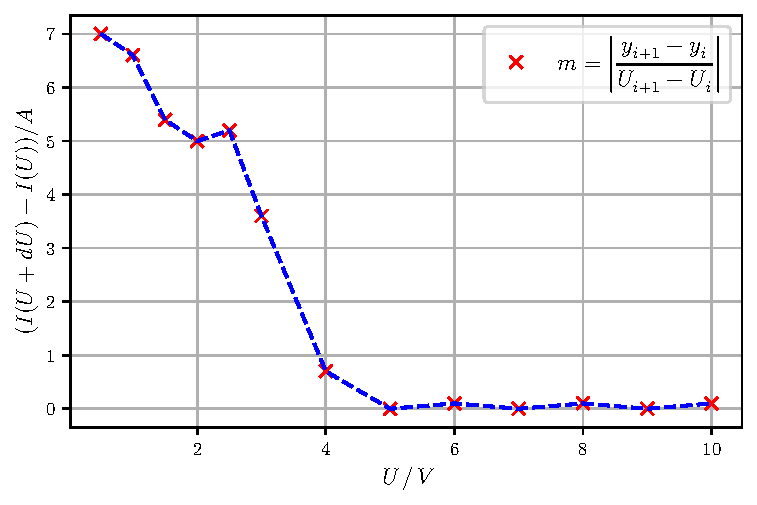
\includegraphics[width=\linewidth]{build/plot2.pdf}
  \captionof{figure}{Die Steigung in Abhängigkeit der Spannung.}
  \label{fig:plot2}
  \end{minipage}
\end{table}


\subsection{Auswertung der Franck-Hertz-Kurven}

Im Folgenden werden die Messdaten aus \autoref{fig:kurve3} und \autoref{fig:kurve4} ausgewertet.
Aus diesen Messungen, die ebenfalls vom XY-Schreiber aufgenommen wurden, werden die Maxima entnommen.
Die ausgewerteten Messwerte dazu sind in \autoref{tab:tabelle4} eingetragen.

\begin{table} [H]
  \centering
  \caption{Abstand vom Nullpunkt der beiden Messungen}
  \label{tab:tabelle4}
  \begin{tabular}{c c c}
      \toprule
      i-tes Maximum &  T = \qty{448.35}{°K}: $U_i - U_{i-1}$ & T = \qty{459.05}{°K}: $U_i - U_{i-1}$\\
      \midrule 
      1 & 7,30 & 6,92 \\
      2 & 4,62 & 4,62 \\
      3 & 5,00 & 5,34 \\
      4 & 5,39 & 5,00 \\
      5 & 5,39 & 5,39 \\
      6 & 5,00 & 5,01 \\
      7 & 5,77 & 6,55 \\
      \bottomrule
  \end{tabular}
\end{table}


Gemittelt ergibt sich dann
\begin{align*}
  T = 448,35 \unit\K: \increment U_1 &= \num{5.5(8)}  &\implies E = \qty{5.5(8)}{eV} \\
  \shortintertext{und}
  T = 459,05 \unit\K: \increment U_2 &= \num{5.5(8)}  &\implies E = \qty{5.5(8)}{eV} \, .
\end{align*}
Daraus lässt sich nun mit \autoref{eq:lambda} die experimentell ermittelte Wellenlänge des emittierten Lichtquants bestimmen.
Es folgt
\begin{align*}
  \lambda_1 &= \qty{226(3)}{nm} \\
  \shortintertext{und}
  \lambda_2 &= \qty{224(32)}{nm} \. .
\end{align*}